\section*{Задача 980}
Найти и исследовать особые точки.
$$
    y' = {2x + y}{x - 2y - 5}
$$

\begin{solution}
    $$\begin{cases}
            2x + y = 0 \\
            x - 2y - 5 = 0
        \end{cases} => x = 1, y = -2 $$
    Запишем матрицу 1-го приближения:
    $$ \tilde{A} = \begin{pmatrix}
            1 & -2 \\
            2 & 1
        \end{pmatrix} $$
    $$ |\tilde{A} - \lambda E| = \begin{vmatrix}
            1 - \lambda & -2          \\
            2           & 1 - \lambda
        \end{vmatrix} = (1 - \lambda)^2 + 4 = 0 $$
    $$ \lambda^2 - 2\lambda + 5 = 0 => $$
    $$ => \lambda_{1, 2} = 1 \pm 2 \cdot i => $$
    => фокус.
    \begin{figure}[h]
        \centering
        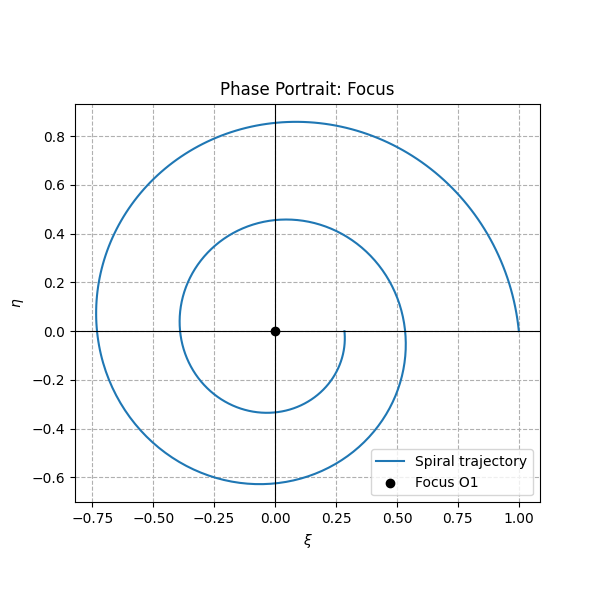
\includegraphics[width=0.8\linewidth]{graph/980.png}
    \end{figure}
\end{solution}